% ============================================================
%  CHAPTER 29: ELECTRONICS
%  The Physics Codex: A Complete University Foundation
%  Korede Samuel Omotosho (Falcon)
%  Aurikrex Learning Systems, 2026
%
%  File: chapters/part5/ch29_electronics.tex
% ============================================================

\chapter{Electronics}
\label{ch:electronics}
\minitoc
\newpage

\chapterquote{The computer was born to solve problems
that did not exist before.}{Bill Gates}

\begin{objectivebox}
By the end of this chapter, you should be able to:
\begin{enumerate}[noitemsep]
  \item Describe the structure and properties of
  semiconductors, including the role of doping
  \item Distinguish between $p$-type and $n$-type
  semiconductors
  \item Describe the $p$-$n$ junction and its
  behaviour under forward and reverse bias
  \item Describe and apply the semiconductor diode,
  including rectification circuits
  \item Describe the transistor and its operation
  as a switch and amplifier
  \item Define and apply current and voltage gain
  \item Describe the light-emitting diode (LED),
  photodiode and thermistor
  \item Describe the operation of the operational
  amplifier (op-amp) in inverting and
  non-inverting configurations
  \item Apply op-amp gain formulae
  \item Describe basic logic gates and construct
  truth tables
\end{enumerate}
\end{objectivebox}

% ============================================================
\section{Intuition: The Transistor Changed Everything}
% ============================================================

Before December 1947, computers filled entire rooms,
ran on hundreds of vacuum tubes (each the size of a
light bulb), consumed kilowatts of power, and failed
frequently as tubes burned out. On December 23, 1947,
John Bardeen, Walter Brattain and William Shockley at
Bell Labs demonstrated the first transistor.

Sixty years later, a single silicon chip the size of
a fingernail contains over a billion transistors. Your
smartphone contains more computing power than all the
computers that existed in 1960, combined.

The transistor is built from \textbf{semiconductor}
material --- specifically silicon, engineered at the
atomic level by introducing tiny concentrations of
impurities. Understanding semiconductors means
understanding why the modern world is possible.

% ============================================================
\section{Semiconductors}
% ============================================================

\begin{definitionbox}[Conductors, Semiconductors and Insulators]
The electrical conductivity of materials spans
roughly 25 orders of magnitude. The classification:

\textbf{Conductors:} $\sigma \sim 10^7\ \Omega^{-1}\text{m}^{-1}$
(copper, aluminium). Free electrons available at
all temperatures.

\textbf{Semiconductors:} $\sigma \sim 10^{-3}$
to $10^4\ \Omega^{-1}\text{m}^{-1}$ (silicon,
germanium). Very few charge carriers at room
temperature; conductivity increases dramatically
with temperature or light.

\textbf{Insulators:} $\sigma \sim 10^{-15}\ \Omega^{-1}\text{m}^{-1}$
(glass, rubber). Negligible free carriers.
\end{definitionbox}

\begin{processbox}[The Semiconductor Band Model]
In a silicon crystal, each atom forms four covalent
bonds with its neighbours. At absolute zero, all
electrons are in bonds --- the \textbf{valence band}
is full and the \textbf{conduction band} is empty.
There is an energy gap (band gap) of $\sim 1.1\ \text{eV}$
between them.

At room temperature, thermal energy occasionally
frees an electron from a bond, promoting it to the
conduction band. This leaves a \textbf{hole} ---
a vacancy in the valence band that behaves as a
mobile positive charge. Both the electron and the
hole contribute to conduction.

In a pure (\textbf{intrinsic}) semiconductor, the
number of conduction electrons equals the number of
holes. Conductivity is low but increases rapidly
with temperature.
\end{processbox}

% ============================================================
\section{Doping}
% ============================================================

\begin{definitionbox}[Doping and Extrinsic Semiconductors]
\textbf{Doping} is the deliberate introduction of
a tiny concentration of impurity atoms into a
pure semiconductor to dramatically increase its
conductivity and control the type of charge carrier.

\textbf{$n$-type semiconductor:} Doped with a
\textbf{pentavalent} (Group V) impurity such as
phosphorus or arsenic. Each impurity atom has 5
valence electrons; 4 form bonds with silicon
neighbours; the 5th is weakly bound and easily
freed as a conduction electron. Majority carriers:
electrons.

\textbf{$p$-type semiconductor:} Doped with a
\textbf{trivalent} (Group III) impurity such as
boron or aluminium. Each impurity atom has 3
valence electrons; it can only form 3 bonds,
leaving one bond site vacant. This vacancy acts
as a hole --- easily filled by a neighbouring
electron, which leaves a hole behind it, making
holes mobile. Majority carriers: holes.

In both types, the semiconductor remains
electrically neutral overall.
\end{definitionbox}

\begin{diagbox}[$n$-type and $p$-type Silicon Crystals]
\begin{center}
\begin{tikzpicture}[scale=0.9, font=\small]

  % === n-TYPE ===
  \begin{scope}[shift={(0,0)}]
    \node[font=\bfseries, codexblue] at (3.5,6.0)
      {$n$-type (phosphorus in silicon)};

    % Silicon lattice (4x4 grid)
    \foreach \x in {0.5,1.5,2.5,3.5,4.5,5.5} {
      \foreach \y in {0.5,1.5,2.5,3.5,4.5} {
        \fill[gray!40] (\x,\y) circle (0.3);
        \node[white, font=\tiny] at (\x,\y) {Si};
      }
    }
    % Bonds (horizontal)
    \foreach \x in {0.8,1.8,2.8,3.8,4.8} {
      \foreach \y in {0.5,1.5,2.5,3.5,4.5} {
        \draw[gray!50, thin] (\x,\y) -- (\x+0.4,\y);
      }
    }
    % Bonds (vertical)
    \foreach \x in {0.5,1.5,2.5,3.5,4.5,5.5} {
      \foreach \y in {0.8,1.8,2.8,3.8} {
        \draw[gray!50, thin] (\x,\y) -- (\x,\y+0.4);
      }
    }

    % Phosphorus impurity (at 3,2.5)
    \fill[codexblue!70] (3.5,2.5) circle (0.35);
    \node[white, font=\tiny] at (3.5,2.5) {P};

    % Free electron
    \fill[codexblue] (3.5,3.8) circle (0.15);
    \draw[->, thick, codexblue]
      (3.5,2.9) -- (3.5,3.6);
    \node[right, codexblue, font=\tiny] at (3.7,3.6)
      {Free $e^-$};

    % Label
    \node[codexblue, font=\small] at (3.5,-0.2)
      {Majority carriers: electrons ($e^-$)};
  \end{scope}

  % === p-TYPE ===
  \begin{scope}[shift={(8,0)}]
    \node[font=\bfseries, codexred] at (3.5,6.0)
      {$p$-type (boron in silicon)};

    % Silicon lattice
    \foreach \x in {0.5,1.5,2.5,3.5,4.5,5.5} {
      \foreach \y in {0.5,1.5,2.5,3.5,4.5} {
        \fill[gray!40] (\x,\y) circle (0.3);
        \node[white, font=\tiny] at (\x,\y) {Si};
      }
    }
    \foreach \x in {0.8,1.8,2.8,3.8,4.8} {
      \foreach \y in {0.5,1.5,2.5,3.5,4.5} {
        \draw[gray!50, thin] (\x,\y) -- (\x+0.4,\y);
      }
    }
    \foreach \x in {0.5,1.5,2.5,3.5,4.5,5.5} {
      \foreach \y in {0.8,1.8,2.8,3.8} {
        \draw[gray!50, thin] (\x,\y) -- (\x,\y+0.4);
      }
    }

    % Boron impurity
    \fill[codexred!70] (3.5,2.5) circle (0.35);
    \node[white, font=\tiny] at (3.5,2.5) {B};

    % Hole (empty circle)
    \draw[thick, codexred] (4.5,2.5) circle (0.25);
    \node[codexred, font=\small] at (4.5,2.5) {$+$};
    \draw[->, thick, codexred]
      (3.9,2.5) -- (4.2,2.5);
    \node[above, codexred, font=\tiny] at (4.5,2.8)
      {Hole};

    % Label
    \node[codexred, font=\small] at (3.5,-0.2)
      {Majority carriers: holes ($h^+$)};
  \end{scope}

\end{tikzpicture}
\end{center}
\end{diagbox}

% ============================================================
\section{The $p$-$n$ Junction}
% ============================================================

When $p$-type and $n$-type semiconductors are joined,
a $p$-$n$ junction forms. This is the basis of all
modern electronic devices.

\begin{processbox}[Formation of the Depletion Region]
At the junction, electrons from the $n$-side diffuse
toward the $p$-side, and holes from the $p$-side
diffuse toward the $n$-side. Near the junction they
meet and recombine --- electrons fill holes.

This leaves a region depleted of mobile charge
carriers called the \textbf{depletion region}
(depletion layer). In this region, the $n$-side
has fixed positive ions (donor atoms that lost their
free electron) and the $p$-side has fixed negative
ions (acceptor atoms that gained an electron).

This creates a built-in \textbf{potential barrier}
(contact potential, $\sim 0.6\ \text{V}$ for silicon,
$0.3\ \text{V}$ for germanium) that prevents further
diffusion.
\end{processbox}

\begin{lawbox}[Forward and Reverse Bias]
\textbf{Forward bias:} Positive terminal of battery
connected to $p$-side, negative to $n$-side.
The external voltage opposes and narrows the depletion
region. When $V > V_{barrier}$ ($\approx 0.6\ \text{V}$
for Si), current flows freely. The diode \textbf{conducts}.

\textbf{Reverse bias:} Positive terminal connected to
$n$-side, negative to $p$-side.
The external voltage widens the depletion region.
Only a tiny \textbf{leakage current} flows (minority
carriers). The diode is essentially \textbf{non-conducting}.
\end{lawbox}

\begin{diagbox}[$p$-$n$ Junction Diode: Forward and Reverse Bias]
\begin{center}
\begin{tikzpicture}[scale=0.9, font=\small]

  % === FORWARD BIAS ===
  \begin{scope}[shift={(0,0)}]
    \node[font=\bfseries, codexblue] at (3.0,5.5)
      {Forward Bias: Conducts};

    % $p$-type (left)
    \fill[codexred!20] (0,1.5) rectangle (2.5,4.5);
    \draw[thick] (0,1.5) rectangle (2.5,4.5);
    \node[codexred, font=\small] at (1.25,3.5) {$p$-type};
    \foreach \x in {0.5,1.0,1.5,2.0} {
      \foreach \y in {2.0,2.5,3.0,3.5,4.0} {
        \node[codexred, font=\small] at (\x,\y) {$+$};
      }
    }

    % $n$-type (right)
    \fill[codexblue!20] (3.5,1.5) rectangle (6.0,4.5);
    \draw[thick] (3.5,1.5) rectangle (6.0,4.5);
    \node[codexblue, font=\small] at (4.75,3.5) {$n$-type};
    \foreach \x in {4.0,4.5,5.0,5.5} {
      \foreach \y in {2.0,2.5,3.0,3.5,4.0} {
        \fill[codexblue] (\x,\y) circle (3pt);
      }
    }

    % Narrow depletion region
    \fill[gray!40] (2.5,1.5) rectangle (3.5,4.5);
    \draw[thick] (2.5,1.5) -- (2.5,4.5);
    \draw[thick] (3.5,1.5) -- (3.5,4.5);
    \node[gray, font=\tiny, rotate=90]
      at (3.0,3.0) {Depletion\\region\\(narrow)};

    % Battery
    \draw[thick] (0,3.0) -- (-1.5,3.0);
    \draw[thick] (6.0,3.0) -- (7.5,3.0);
    \draw[thick] (-1.5,3.0) -- (-1.5,0.5);
    \draw[thick] (7.5,3.0) -- (7.5,0.5);
    \draw[thick] (-1.5,0.5) -- (7.5,0.5);
    % Battery symbol
    \draw[very thick, codexred] (2.5,0.5) -- (3.5,0.5);
    \draw[very thick] (2.0,0.3) -- (4.0,0.3);
    \node[above, codexred, font=\small] at (2.5,0.6)
      {$+$};
    \node[above, codexblue, font=\small] at (4.5,0.6)
      {$-$};

    % Current flow (large)
    \draw[->, very thick, codexblue, line width=2pt]
      (6.5,3.0) -- (5.5,3.0);
    \draw[->, very thick, codexblue, line width=2pt]
      (0.5,3.0) -- (-0.5,3.0);
    \node[codexblue, font=\small] at (3.0,5.0)
      {Large current $\Rightarrow$ Low resistance};
  \end{scope}

  % === REVERSE BIAS ===
  \begin{scope}[shift={(9.5,0)}]
    \node[font=\bfseries, codexred] at (3.0,5.5)
      {Reverse Bias: Non-conducting};

    % Same structure but wider depletion region
    \fill[codexred!20] (0,1.5) rectangle (2.0,4.5);
    \draw[thick] (0,1.5) rectangle (2.0,4.5);
    \node[codexred, font=\small] at (1.0,3.0) {$p$-type};

    \fill[codexblue!20] (4.0,1.5) rectangle (6.0,4.5);
    \draw[thick] (4.0,1.5) rectangle (6.0,4.5);
    \node[codexblue, font=\small] at (5.0,3.0) {$n$-type};

    % Wide depletion region
    \fill[gray!40] (2.0,1.5) rectangle (4.0,4.5);
    \draw[thick] (2.0,1.5) -- (2.0,4.5);
    \draw[thick] (4.0,1.5) -- (4.0,4.5);
    \node[gray, font=\tiny, rotate=90]
      at (3.0,3.0) {Wide depletion region};

    % Battery (reversed polarity)
    \draw[thick] (0,3.0) -- (-1.5,3.0);
    \draw[thick] (6.0,3.0) -- (7.5,3.0);
    \draw[thick] (-1.5,3.0) -- (-1.5,0.5);
    \draw[thick] (7.5,3.0) -- (7.5,0.5);
    \draw[thick] (-1.5,0.5) -- (7.5,0.5);
    % Battery reversed
    \draw[very thick, codexblue] (2.5,0.5) -- (3.5,0.5);
    \draw[very thick] (2.0,0.3) -- (4.0,0.3);
    \node[above, codexblue, font=\small] at (2.3,0.6)
      {$-$};
    \node[above, codexred, font=\small] at (4.5,0.6)
      {$+$};

    % Tiny leakage current only
    \draw[->, thin, gray]
      (6.5,3.0) -- (6.0,3.0);
    \node[gray, font=\small] at (3.0,5.0)
      {Tiny leakage current $\Rightarrow$ High resistance};
  \end{scope}

\end{tikzpicture}
\end{center}
\end{diagbox}

% ============================================================
\section{The Semiconductor Diode}
% ============================================================

\begin{definitionbox}[Diode Characteristics]
A semiconductor diode allows current to flow freely
in one direction (forward bias) and blocks it in
the other direction (reverse bias).

The forward voltage drop across a conducting silicon
diode is approximately $0.6$--$0.7\ \text{V}$ (silicon)
or $0.2$--$0.3\ \text{V}$ (germanium).

\textbf{Diode symbol:}
\begin{center}
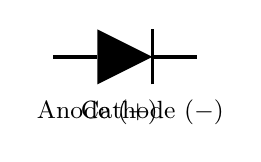
\begin{tikzpicture}[scale=0.7]
  \draw[very thick] (0,0) -- (0.8,0);
  % Triangle pointing right
  \fill[black] (0.8,-0.5) -- (0.8,0.5) -- (1.8,0) -- cycle;
  % Bar
  \draw[very thick] (1.8,-0.5) -- (1.8,0.5);
  \draw[very thick] (1.8,0) -- (2.6,0);
  % Anode/Cathode labels
  \node[below, font=\small] at (0.8,-0.6) {Anode ($+$)};
  \node[below, font=\small] at (1.8,-0.6) {Cathode ($-$)};
\end{tikzpicture}
\end{center}
Current flows in the direction the triangle points
(from anode to cathode in forward bias).
\end{definitionbox}

\subsection{Half-Wave Rectification}

\begin{processbox}[Half-Wave Rectification]
A single diode in series with a load resistor allows
only the positive half-cycles of an AC supply to pass,
blocking the negative half-cycles. The output is a
pulsating DC (only positive half-cycles). Half the
input energy is wasted.
\end{processbox}

\subsection{Full-Wave Rectification: Bridge Rectifier}

\begin{processbox}[Full-Wave Bridge Rectifier]
Four diodes arranged in a diamond (bridge) convert
both half-cycles of AC to the same polarity of DC.
During the positive half-cycle, current flows through
two diodes; during the negative half-cycle, through
the other two. The output always flows in the same
direction through the load.

The output is a full-wave pulsating DC. Adding a
smoothing capacitor in parallel with the load
reduces the ripple and gives a nearly constant DC.
\end{processbox}

\begin{diagbox}[Half-Wave and Full-Wave Rectification Circuits and Waveforms]
\begin{center}
\begin{tikzpicture}

  % HALF-WAVE
  \begin{scope}[shift={(0,5)}]
    \node[font=\bfseries] at (3.5,2.5)
      {Half-Wave Rectifier};
    % AC input (simple representation)
    \draw[thick] (0,1.5) -- (0.5,1.5);
    \draw[thick, codexblue]
      (0.5,1.5) .. controls (0.7,2.2) and (0.9,2.2)
      .. (1.1,1.5)
      .. controls (1.3,0.8) and (1.5,0.8)
      .. (1.7,1.5);
    % Diode
    \fill[black] (2.2,1.0) -- (2.2,2.0) -- (3.2,1.5)
      -- cycle;
    \draw[thick] (3.2,1.0) -- (3.2,2.0);
    \draw[thick] (1.7,1.5) -- (2.2,1.5);
    \draw[thick] (3.2,1.5) -- (4.0,1.5);
    % Load
    \fill[gray!30] (4.0,1.0) rectangle (4.5,2.0);
    \draw[thick] (4.0,1.0) rectangle (4.5,2.0);
    \node[font=\tiny] at (4.25,1.5) {$R$};
    \draw[thick] (0,1.5) -- (0,0.5) -- (4.25,0.5)
      -- (4.25,1.0);
    \draw[thick] (4.25,2.0) -- (4.25,2.5)
      -- (4.5,2.5);
  \end{scope}

  % FULL-WAVE
  \begin{scope}[shift={(7,5)}]
    \node[font=\bfseries] at (3.0,3.2)
      {Full-Wave Bridge Rectifier};
    % Bridge circuit (simplified)
    \coordinate (L) at (0,1.5);
    \coordinate (T) at (2.0,3.0);
    \coordinate (R) at (4.0,1.5);
    \coordinate (B) at (2.0,0);
    % Diodes on four arms
    \draw[thick] (L) -- (T);
    \draw[thick] (T) -- (R);
    \draw[thick] (R) -- (B);
    \draw[thick] (B) -- (L);
    % Diode arrows on each arm
    % Left-top: current up-right
    \fill[black] (0.7,2.1) -- (0.5,1.9) -- (1.3,2.7)
      -- cycle;
    % Right-top: current down-left
    \fill[black] (3.3,2.7) -- (2.7,2.1) -- (3.5,1.9)
      -- cycle;
    % Left-bottom
    \fill[black] (0.5,1.1) -- (0.7,0.9) -- (1.3,0.3)
      -- cycle;
    % Right-bottom
    \fill[black] (3.3,0.3) -- (2.7,0.9) -- (3.5,1.1)
      -- cycle;
    % AC input
    \draw[thick, codexblue] (-1.0,1.5) -- (0,1.5);
    \draw[thick, codexblue] (4.0,1.5) -- (5.0,1.5);
    \node[left, codexblue, font=\tiny] at (-1.0,1.5)
      {AC in};
    % DC output (top-bottom)
    \draw[thick, codexred] (2.0,3.0) -- (2.0,4.0);
    \draw[thick, codexred] (2.0,0) -- (2.0,-0.8);
    \node[above, codexred, font=\tiny] at (2.0,4.0)
      {$+$};
    \node[below, codexred, font=\tiny] at (2.0,-0.8)
      {$-$};
    \node[right, codexred, font=\tiny] at (2.2,2.0)
      {DC out};
  \end{scope}

  % WAVEFORM COMPARISON
  \begin{axis}[
    name=wave1,
    at={(0pt,0pt)},
    width=7cm, height=3.5cm,
    title={Input AC},
    xlabel={}, ylabel={$V$},
    xmin=0, xmax=4*pi,
    ymin=-1.2, ymax=1.2,
    xtick=\empty, ytick={-1,0,1},
    yticklabels={$-V_0$,0,$+V_0$},
    grid=major, grid style={gray!15},
  ]
    \addplot[codexblue, thick, domain=0:4*pi,
      samples=150]{sin(deg(x))};
  \end{axis}

  \begin{axis}[
    name=wave2,
    at={(wave1.right of south east)},
    anchor=left of south west,
    xshift=0.2cm,
    width=7cm, height=3.5cm,
    title={Half-wave output},
    xlabel={}, ylabel={$V$},
    xmin=0, xmax=4*pi,
    ymin=-1.2, ymax=1.2,
    xtick=\empty, ytick={0,1},
    yticklabels={0,$+V_0$},
    grid=major, grid style={gray!15},
  ]
    % Only positive halves
    \addplot[codexred, thick, domain=0:pi,
      samples=80]{sin(deg(x))};
    \addplot[codexred, thick, domain=pi:2*pi]
      {0};
    \addplot[codexred, thick, domain=2*pi:3*pi,
      samples=80]{sin(deg(x))};
    \addplot[codexred, thick, domain=3*pi:4*pi]
      {0};
  \end{axis}

  \begin{axis}[
    name=wave3,
    at={(wave2.right of south east)},
    anchor=left of south west,
    xshift=0.2cm,
    width=7cm, height=3.5cm,
    title={Full-wave output},
    xlabel={Time}, ylabel={$V$},
    xmin=0, xmax=4*pi,
    ymin=-0.1, ymax=1.2,
    xtick=\empty, ytick={0,1},
    yticklabels={0,$+V_0$},
    grid=major, grid style={gray!15},
  ]
    \addplot[codexgreen, thick, domain=0:4*pi,
      samples=150]{abs(sin(deg(x)))};
  \end{axis}

\end{tikzpicture}
\end{center}
\end{diagbox}

% ============================================================
\section{Special Diodes}
% ============================================================

\begin{defbox}[Light-Emitting Diode (LED)]
An \textbf{LED} emits photons when forward biased.
Electrons crossing the junction recombine with holes,
releasing energy as photons. The colour (wavelength)
depends on the band gap of the semiconductor material.

LEDs are used for displays, indicator lights,
traffic lights, and (high-power variants) for
general illumination. They are far more efficient
than incandescent bulbs ($\sim 50$--$150\ \text{lm/W}$
vs $\sim 15\ \text{lm/W}$). All LED bulbs in use
across Nigeria contain $p$-$n$ junctions operating
exactly as described here.
\end{defbox}

\begin{defbox}[Photodiode]
A \textbf{photodiode} is operated in reverse bias.
When photons of sufficient energy fall on the
depletion region, they create electron-hole pairs
(photogeneration). These carriers are swept across
the junction by the built-in electric field, producing
a current proportional to the light intensity. Used
in light meters, optical fibre receivers, barcode
scanners, and solar cells.
\end{defbox}

% ============================================================
\section{The Transistor}
% ============================================================

\begin{definitionbox}[The Bipolar Junction Transistor (BJT)]
A transistor consists of three layers of semiconductor:
either $n$-$p$-$n$ or $p$-$n$-$p$. The three
regions are called the \textbf{emitter} (E),
\textbf{base} (B), and \textbf{collector} (C).

The base is very thin ($\sim 1\ \mu\text{m}$) and
lightly doped.

In an \textbf{$n$-$p$-$n$} transistor (the most
common type):
\begin{itemize}[noitemsep]
  \item The base-emitter junction is forward biased
  (small $V_{BE} \approx 0.6\ \text{V}$)
  \item The base-collector junction is reverse biased
  \item Electrons injected from emitter into the thin
  base mostly diffuse through to the collector
  (rather than recombining with holes in the base)
  \item A small base current $I_B$ controls a much
  larger collector current $I_C$
\end{itemize}
\end{definitionbox}

\begin{lawbox}[Transistor Equations]
For a BJT:
\[
  I_E = I_B + I_C
\]
The \textbf{current gain} $h_{FE}$ (or $\beta$):
\[
  h_{FE} = \frac{I_C}{I_B}
  \quad (\text{typically } 50 \text{ to } 500)
\]
So: $I_C = h_{FE}\,I_B$

\textbf{Voltage gain} of a common-emitter amplifier:
\[
  A_v = -\frac{R_C}{R_E}
  \approx -\frac{V_{out}}{V_{in}}
\]
The negative sign indicates phase inversion --- output
is $180°$ out of phase with input.
\end{lawbox}

\begin{diagbox}[$n$-$p$-$n$ Transistor as Switch and Amplifier]
\begin{center}
\begin{tikzpicture}[scale=0.9, font=\small]

  % === TRANSISTOR AS SWITCH ===
  \begin{scope}[shift={(0,0)}]
    \node[font=\bfseries] at (3.0,6.5)
      {Transistor Switch};

    % Power supply rail
    \draw[very thick] (0,6.0) -- (6.0,6.0);
    \node[above] at (3.0,6.1) {$+V_{CC}$};

    % Collector resistor R_C
    \fill[gray!30] (2.5,4.8) rectangle (3.5,6.0);
    \draw[thick] (2.5,4.8) rectangle (3.5,6.0);
    \node[right, font=\small] at (3.6,5.4) {$R_C$};
    \draw[thick] (3.0,6.0) -- (3.0,4.8);

    % Transistor symbol
    % Collector
    \draw[thick] (3.0,4.8) -- (3.0,4.2);
    % Base line
    \draw[very thick] (3.0,3.5) -- (3.0,4.2);
    \draw[very thick] (3.0,3.5) -- (3.0,2.8);
    % Emitter (with arrow for npn)
    \draw[thick] (3.0,2.8) -- (3.0,2.2);
    % Collector terminal
    \draw[thick] (3.0,4.0) -- (4.0,4.5);
    % Emitter terminal (with arrow)
    \draw[thick] (3.0,3.0) -- (4.0,2.5);
    \draw[->, thick] (3.7,2.7) -- (4.0,2.5);
    % Base terminal
    \draw[thick] (3.0,3.5) -- (1.5,3.5);
    % Labels
    \node[above, font=\small] at (4.0,4.5) {C};
    \node[below, font=\small] at (4.0,2.5) {E};
    \node[left, font=\small] at (1.4,3.5) {B};

    % Ground
    \draw[thick] (3.0,2.2) -- (3.0,1.5);
    \draw[thick] (2.5,1.5) -- (3.5,1.5);
    \draw[thick] (2.7,1.3) -- (3.3,1.3);
    \draw[thick] (2.9,1.1) -- (3.1,1.1);

    % Base resistor and input
    \fill[gray!30] (0.5,3.2) rectangle (1.2,3.8);
    \draw[thick] (0.5,3.2) rectangle (1.2,3.8);
    \node[above, font=\tiny] at (0.85,3.85) {$R_B$};
    \draw[thick] (0,3.5) -- (0.5,3.5);
    \draw[thick] (1.2,3.5) -- (1.5,3.5);
    \node[left, font=\small] at (-0.1,3.5)
      {$V_{in}$};

    % Output (collector)
    \draw[thick, dashed] (4.0,4.5) -- (5.5,4.5);
    \node[right, font=\small] at (5.6,4.5)
      {$V_{out}$};

    % State table
    \node[align=left, font=\small, draw=gray,
      rounded corners, fill=white, inner sep=4pt]
      at (3.0,-0.5)
      {$V_{in}$ low: $I_B=0$, $I_C=0$,\\
      \quad transistor OFF, $V_{out}=V_{CC}$\\
      $V_{in}$ high: $I_B>0$, $I_C=h_{FE}I_B$,\\
      \quad transistor ON, $V_{out}\approx 0$};
  \end{scope}

  % === TRANSISTOR AS AMPLIFIER ===
  \begin{scope}[shift={(9,0)}]
    \node[font=\bfseries] at (3.0,6.5)
      {Common-Emitter Amplifier};

    % Power supply
    \draw[very thick] (0,6.0) -- (6.0,6.0);
    \node[above] at (3.0,6.1) {$+V_{CC}$};

    % Collector resistor
    \fill[gray!30] (2.5,4.8) rectangle (3.5,6.0);
    \draw[thick] (2.5,4.8) rectangle (3.5,6.0);
    \node[right, font=\small] at (3.6,5.4) {$R_C$};
    \draw[thick] (3.0,6.0) -- (3.0,4.8);

    % Transistor
    \draw[very thick] (3.0,3.5) -- (3.0,4.2);
    \draw[very thick] (3.0,3.5) -- (3.0,2.8);
    \draw[thick] (3.0,4.0) -- (4.0,4.5);
    \draw[thick] (3.0,3.0) -- (4.0,2.5);
    \draw[->, thick] (3.7,2.7) -- (4.0,2.5);
    \draw[thick] (3.0,3.5) -- (1.5,3.5);
    \node[above, font=\small] at (4.0,4.5) {C};
    \node[below, font=\small] at (4.0,2.5) {E};
    \node[left, font=\small] at (1.4,3.5) {B};

    % Emitter resistor
    \fill[gray!30] (2.5,1.5) rectangle (3.5,2.3);
    \draw[thick] (2.5,1.5) rectangle (3.5,2.3);
    \node[right, font=\small] at (3.6,1.9) {$R_E$};
    \draw[thick] (3.0,2.3) -- (4.0,2.5);
    \draw[thick] (3.0,2.3) -- (3.0,1.5);

    % Ground
    \draw[thick] (3.0,1.5) -- (3.0,1.0);
    \draw[thick] (2.6,1.0) -- (3.4,1.0);
    \draw[thick] (2.8,0.8) -- (3.2,0.8);

    % Input (AC signal at base)
    \draw[thick] (0,3.5) -- (1.5,3.5);
    \draw[codexblue, thick]
      (-0.5,3.5) sin (-0.25,4.0)
      cos (0,3.5) sin (0.25,3.0) cos (0.5,3.5);
    \node[left, codexblue, font=\small]
      at (-0.6,3.5) {$v_{in}$};

    % Output (inverted, amplified AC)
    \draw[thick, dashed] (4.0,4.5) -- (5.5,4.5);
    \draw[codexred, thick]
      (5.5,4.5) sin (5.75,3.5)
      cos (6.0,4.5) sin (6.25,5.5) cos (6.5,4.5);
    \node[right, codexred, font=\small]
      at (6.6,4.5) {$v_{out}$\\(amplified,\\inverted)};

    % Gain formula
    \node[align=center, font=\small] at (3.0,-0.5)
      {$A_v \approx -R_C/R_E$};
  \end{scope}

\end{tikzpicture}
\end{center}
\end{diagbox}

\begin{examplebox}[29.1]
\stepcounter{workedexample}
An $n$-$p$-$n$ transistor has $h_{FE} = 120$.
It is used in a circuit where $R_C = 4.7\ \text{k}\Omega$
and $R_E = 470\ \Omega$.\\
(a) If the base current is $40\ \mu\text{A}$, find
the collector current.\\
(b) Find the emitter current.\\
(c) Find the voltage gain of the amplifier.\\
(d) If the input signal is $50\ \text{mV}$ peak,
find the output voltage.
\end{examplebox}

\begin{solutionbox}
\textbf{(a)} Collector current:
\[
  I_C = h_{FE} \times I_B = 120 \times 40\times10^{-6}
  = 4.8\times10^{-3}\ \text{A} = 4.8\ \text{mA}
\]

\textbf{(b)} Emitter current:
\[
  I_E = I_B + I_C = 0.040 + 4.8 = 4.84\ \text{mA}
\]

\textbf{(c)} Voltage gain:
\[
  A_v = -\frac{R_C}{R_E} = -\frac{4700}{470} = -10
\]

\textbf{(d)} Output voltage (magnitude):
\[
  V_{out} = |A_v| \times V_{in}
  = 10 \times 50\ \text{mV} = 500\ \text{mV}
  = 0.50\ \text{V}
\]
The output is $0.50\ \text{V}$ peak, $180°$ out of
phase with the input (inverted).
\end{solutionbox}

% ============================================================
\section{The Operational Amplifier}
% ============================================================

\begin{definitionbox}[The Operational Amplifier (Op-Amp)]
An \textbf{operational amplifier} is an integrated
circuit containing many transistors, designed to
amplify the voltage \textit{difference} between
two input terminals.

The two inputs are:
\begin{itemize}[noitemsep]
  \item \textbf{Inverting input} ($-$): output
  is inverted (phase-shifted by $180°$) relative
  to a signal applied here.
  \item \textbf{Non-inverting input} ($+$): output
  is in phase with a signal applied here.
\end{itemize}

\textbf{Ideal op-amp properties:}
\begin{itemize}[noitemsep]
  \item Infinite open-loop gain ($A_{OL} \to \infty$)
  \item Infinite input impedance (draws no current)
  \item Zero output impedance
  \item Infinite bandwidth
\end{itemize}
Open-loop gain is so large ($\sim 10^5$--$10^6$)
that the op-amp is almost always used with
\textbf{negative feedback}.
\end{definitionbox}

\begin{lawbox}[Inverting Amplifier]
With a feedback resistor $R_f$ and input resistor
$R_{in}$, the closed-loop gain is:
\[
  A_v = -\frac{R_f}{R_{in}}
\]
The output is inverted. The gain magnitude is
determined only by the resistor ratio (not the
op-amp's internal properties).
\end{lawbox}

\begin{lawbox}[Non-Inverting Amplifier]
With feedback resistor $R_f$ and resistor $R_1$
from inverting input to ground:
\[
  A_v = 1 + \frac{R_f}{R_1}
\]
The output is in phase with the input. Note:
$A_v \geq 1$ always.

\textbf{Voltage follower (unity gain):} $R_f = 0$,
$R_1 = \infty$ (or $R_1$ absent): $A_v = 1$.
Used as a buffer to match impedances.
\end{lawbox}

\begin{diagbox}[Op-Amp Configurations]
\begin{center}
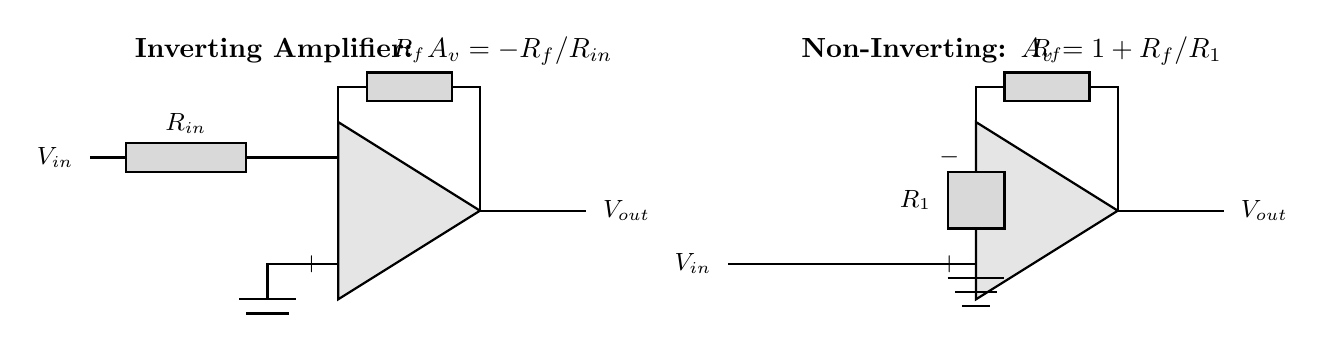
\begin{tikzpicture}[scale=0.9, font=\small]

  % === INVERTING AMPLIFIER ===
  \begin{scope}[shift={(0,0)}]
    \node[font=\bfseries] at (4.0,4.5)
      {Inverting Amplifier: $A_v = -R_f/R_{in}$};

    % Op-amp triangle
    \fill[gray!20]
      (3.5,1.0) -- (3.5,3.5) -- (5.5,2.25) -- cycle;
    \draw[thick]
      (3.5,1.0) -- (3.5,3.5) -- (5.5,2.25) -- cycle;

    % Input labels
    \node[left, font=\small] at (3.4,3.0) {$-$};
    \node[left, font=\small] at (3.4,1.5) {$+$};

    % Input resistor R_in
    \fill[gray!30] (0.5,2.8) rectangle (2.2,3.2);
    \draw[thick] (0.5,2.8) rectangle (2.2,3.2);
    \node[above, font=\small] at (1.35,3.2) {$R_{in}$};
    \draw[thick] (0,3.0) -- (0.5,3.0);
    \draw[thick] (2.2,3.0) -- (3.5,3.0);
    \node[left, font=\small] at (-0.1,3.0) {$V_{in}$};

    % Feedback resistor R_f (top)
    \draw[thick] (3.5,3.0) -- (3.5,4.0)
      -- (5.5,4.0) -- (5.5,2.25);
    \fill[gray!30] (3.9,3.8) rectangle (5.1,4.2);
    \draw[thick] (3.9,3.8) rectangle (5.1,4.2);
    \node[above, font=\small] at (4.5,4.2) {$R_f$};

    % Non-inverting to ground
    \draw[thick] (3.5,1.5) -- (2.5,1.5) -- (2.5,1.0);
    \draw[thick] (2.1,1.0) -- (2.9,1.0);
    \draw[thick] (2.2,0.8) -- (2.8,0.8);

    % Output
    \draw[thick] (5.5,2.25) -- (7.0,2.25);
    \node[right, font=\small] at (7.1,2.25) {$V_{out}$};
  \end{scope}

  % === NON-INVERTING AMPLIFIER ===
  \begin{scope}[shift={(9,0)}]
    \node[font=\bfseries] at (4.0,4.5)
      {Non-Inverting: $A_v = 1 + R_f/R_1$};

    % Op-amp
    \fill[gray!20]
      (3.5,1.0) -- (3.5,3.5) -- (5.5,2.25) -- cycle;
    \draw[thick]
      (3.5,1.0) -- (3.5,3.5) -- (5.5,2.25) -- cycle;
    \node[left, font=\small] at (3.4,3.0) {$-$};
    \node[left, font=\small] at (3.4,1.5) {$+$};

    % Input to non-inverting
    \draw[thick] (0,1.5) -- (3.5,1.5);
    \node[left, font=\small] at (-0.1,1.5) {$V_{in}$};

    % Feedback network (voltage divider R_f, R_1)
    \draw[thick] (5.5,2.25) -- (5.5,4.0)
      -- (3.5,4.0) -- (3.5,3.0);
    \fill[gray!30] (3.9,3.8) rectangle (5.1,4.2);
    \draw[thick] (3.9,3.8) rectangle (5.1,4.2);
    \node[above, font=\small] at (4.5,4.2) {$R_f$};

    % R1 from inverting to ground
    \fill[gray!30] (3.1,2.0) rectangle (3.9,2.8);
    \draw[thick] (3.1,2.0) rectangle (3.9,2.8);
    \node[left, font=\small] at (3.0,2.4) {$R_1$};
    \draw[thick] (3.5,3.0) -- (3.5,2.8);
    \draw[thick] (3.5,2.0) -- (3.5,1.3);
    \draw[thick] (3.1,1.3) -- (3.9,1.3);
    \draw[thick] (3.2,1.1) -- (3.8,1.1);
    \draw[thick] (3.3,0.9) -- (3.7,0.9);

    % Output
    \draw[thick] (5.5,2.25) -- (7.0,2.25);
    \node[right, font=\small] at (7.1,2.25) {$V_{out}$};
  \end{scope}

\end{tikzpicture}
\end{center}
\end{diagbox}

\begin{examplebox}[29.2]
\stepcounter{workedexample}
An inverting op-amp amplifier has $R_{in} = 10\ \text{k}\Omega$
and $R_f = 100\ \text{k}\Omega$. The supply
voltage is $\pm 15\ \text{V}$.\\
(a) Calculate the gain.\\
(b) Find $V_{out}$ when $V_{in} = +0.5\ \text{V}$.\\
(c) Find $V_{out}$ when $V_{in} = +2.0\ \text{V}$.
Explain what happens.\\
(d) Find the value of $R_f$ needed for a gain of
$-25$.
\end{examplebox}

\begin{solutionbox}
\textbf{(a)} Gain:
\[
  A_v = -\frac{R_f}{R_{in}}
  = -\frac{100}{10} = -10
\]

\textbf{(b)} $V_{out} = A_v \times V_{in}
= -10 \times 0.5 = -5.0\ \text{V}$

The output is within the supply rails
($\pm 15\ \text{V}$) --- the op-amp works as expected.

\textbf{(c)} $V_{out} = -10 \times 2.0
= -20\ \text{V}$ (predicted, but impossible).

The output cannot exceed the supply voltage. The
op-amp saturates at approximately $-13\ \text{V}$
(typically $1$--$2\ \text{V}$ below the negative
rail). This is \textbf{clipping} --- the output
is ``clipped'' at the saturation voltage.

\textbf{(d)} For gain $= -25$:
\[
  R_f = 25 \times R_{in} = 25 \times 10
  = 250\ \text{k}\Omega
\]
\end{solutionbox}

% ============================================================
\section{Logic Gates}
% ============================================================

\begin{defbox}[Digital Logic and Logic Gates]
In digital electronics, signals have only two states:
\textbf{HIGH} (logic 1, typically $+5\ \text{V}$ or
$+3.3\ \text{V}$) and \textbf{LOW} (logic 0, typically
$0\ \text{V}$).

A \textbf{logic gate} is a circuit that performs a
Boolean logic operation on one or more inputs and
produces a single output. They are the building
blocks of all computers, processors and digital
systems.
\end{defbox}

\begin{table}[H]
\centering
\caption{Basic Logic Gates: Symbols and Truth Tables}
\label{tab:logic_gates}
\begin{tabular}{p{1.5cm}p{3cm}p{4cm}p{3cm}}
\toprule
\textbf{Gate} & \textbf{Symbol} & \textbf{Truth Table}
& \textbf{Boolean}\\
\midrule
AND & Output HIGH only if ALL inputs HIGH &
  $\begin{array}{ccc}A&B&Q\\0&0&0\\0&1&0\\1&0&0\\1&1&1\end{array}$
  & $Q = A \cdot B$\\[0.5cm]
OR & Output HIGH if ANY input HIGH &
  $\begin{array}{ccc}A&B&Q\\0&0&0\\0&1&1\\1&0&1\\1&1&1\end{array}$
  & $Q = A + B$\\[0.5cm]
NOT & Output is inverse of input &
  $\begin{array}{cc}A&Q\\0&1\\1&0\end{array}$
  & $Q = \bar{A}$\\[0.5cm]
NAND & Inverse of AND &
  $\begin{array}{ccc}A&B&Q\\0&0&1\\0&1&1\\1&0&1\\1&1&0\end{array}$
  & $Q = \overline{A \cdot B}$\\[0.5cm]
NOR & Inverse of OR &
  $\begin{array}{ccc}A&B&Q\\0&0&1\\0&1&0\\1&0&0\\1&1&0\end{array}$
  & $Q = \overline{A + B}$\\[0.5cm]
XOR & Output HIGH if inputs are DIFFERENT &
  $\begin{array}{ccc}A&B&Q\\0&0&0\\0&1&1\\1&0&1\\1&1&0\end{array}$
  & $Q = A \oplus B$\\
\bottomrule
\end{tabular}
\end{table}

\begin{keybox}[NAND and NOR are Universal Gates]
Any Boolean logic function can be built using only
NAND gates (or only NOR gates). These are called
\textbf{universal gates}. This is why most digital
integrated circuits are made predominantly from
NAND gates --- the same fabrication process can
produce any logic function by varying the connections.

A NOT gate is just a NAND with both inputs connected
together. An AND gate is a NAND followed by a NOT.
An OR gate is made from three NANDs.
\end{keybox}

\begin{examplebox}[29.3]
\stepcounter{workedexample}
A burglar alarm system has three sensors: a door
sensor (D), a window sensor (W), and a motion
sensor (M). The alarm output (A) should be HIGH
if D is HIGH OR if both W and M are HIGH.\\
(a) Write the Boolean expression for A.\\
(b) Construct the truth table (8 rows).\\
(c) Design the logic gate circuit.
\end{examplebox}

\begin{solutionbox}
\textbf{(a)} Boolean expression:
\[
  A = D + (W \cdot M)
\]
(D OR (W AND M))

\textbf{(b)} Truth table:
\begin{center}
\begin{tabular}{cccc}
\toprule
D & W & M & A = D + (W·M)\\
\midrule
0 & 0 & 0 & 0\\
0 & 0 & 1 & 0\\
0 & 1 & 0 & 0\\
0 & 1 & 1 & 1 (W AND M)\\
1 & 0 & 0 & 1 (D)\\
1 & 0 & 1 & 1 (D)\\
1 & 1 & 0 & 1 (D)\\
1 & 1 & 1 & 1\\
\bottomrule
\end{tabular}
\end{center}

\textbf{(c)} Circuit: W and M feed into an AND gate,
whose output and D feed into an OR gate, producing A.
\end{solutionbox}

% ============================================================
\section{Chapter Summary}
% ============================================================

\begin{summarybox}
\textbf{Semiconductors:} silicon, germanium.
Conductivity increases with temperature; few charge
carriers at room temperature.

\textbf{Doping:}
$n$-type: pentavalent impurity, majority carriers
are electrons.
$p$-type: trivalent impurity, majority carriers
are holes.

\textbf{$p$-$n$ junction:} depletion region forms.
Forward bias: conducts ($V > 0.6\ \text{V}$ for Si).
Reverse bias: non-conducting.

\textbf{Diode:} current in one direction only.
Used for rectification (half-wave, full-wave bridge).
LED emits photons; photodiode detects photons.

\textbf{BJT transistor:}
$I_C = h_{FE} I_B$; $I_E = I_C + I_B$.
Switch (OFF/ON) or amplifier (voltage gain
$A_v = -R_C/R_E$).

\textbf{Op-amp:}
Inverting: $A_v = -R_f/R_{in}$.
Non-inverting: $A_v = 1 + R_f/R_1$.
Output saturates at supply rail voltage.

\textbf{Logic gates:} AND, OR, NOT, NAND, NOR, XOR.
NAND and NOR are universal.
Truth tables define gate behaviour completely.
\end{summarybox}

% ============================================================
\newpage
\begin{exercisebox}[29]

\subsection*{Section A: Multiple Choice}

\textbf{A1.} An $n$-type semiconductor is formed by
doping silicon with:

\mcoption{A}{A Group III (trivalent) element
such as boron}
\mcoption{B}{A Group V (pentavalent) element
such as phosphorus}
\mcoption{C}{A Group II element}
\mcoption{D}{A Group VI element}
\ansref{Ch29-A1}

\vspace{0.4cm}

\textbf{A2.} In a forward-biased silicon diode,
the approximate voltage drop across the junction is:

\mcoption{A}{$0\ \text{V}$}
\mcoption{B}{$0.3\ \text{V}$}
\mcoption{C}{$0.6\ \text{V}$}
\mcoption{D}{$1.2\ \text{V}$}
\ansref{Ch29-A2}

\vspace{0.4cm}

\textbf{A3.} A transistor has $h_{FE} = 200$ and
$I_B = 25\ \mu\text{A}$. The collector current is:

\mcoption{A}{$0.125\ \text{mA}$}
\mcoption{B}{$1.25\ \text{mA}$}
\mcoption{C}{$5.0\ \text{mA}$}
\mcoption{D}{$50\ \text{mA}$}
\ansref{Ch29-A3}

\vspace{0.4cm}

\textbf{A4.} A full-wave bridge rectifier uses:

\mcoption{A}{One diode}
\mcoption{B}{Two diodes}
\mcoption{C}{Three diodes}
\mcoption{D}{Four diodes}
\ansref{Ch29-A4}

\vspace{0.4cm}

\textbf{A5.} An inverting op-amp has $R_{in}
= 20\ \text{k}\Omega$ and $R_f = 180\ \text{k}\Omega$.
Its voltage gain is:

\mcoption{A}{$+9$}
\mcoption{B}{$-9$}
\mcoption{C}{$+10$}
\mcoption{D}{$-10$}
\ansref{Ch29-A5}

\vspace{0.4cm}

\textbf{A6.} In a common-emitter transistor
amplifier, the output voltage is:

\mcoption{A}{In phase with the input}
\mcoption{B}{$90°$ out of phase with the input}
\mcoption{C}{$180°$ out of phase with the input
(inverted)}
\mcoption{D}{Independent of the input}
\ansref{Ch29-A6}

\vspace{0.4cm}

\textbf{A7.} A NAND gate with inputs A=1 and B=0
produces output:

\mcoption{A}{0}
\mcoption{B}{1}
\mcoption{C}{It depends on the power supply}
\mcoption{D}{Undefined}
\ansref{Ch29-A7}

\vspace{0.4cm}

\textbf{A8.} The depletion region in a $p$-$n$
junction:

\mcoption{A}{Contains mobile charge carriers}
\mcoption{B}{Is depleted of mobile charge carriers}
\mcoption{C}{Widens in forward bias}
\mcoption{D}{Contains no ions}
\ansref{Ch29-A8}

\vspace{0.4cm}

\textbf{A9.} A photodiode is operated in:

\mcoption{A}{Forward bias with no light}
\mcoption{B}{Forward bias with light incident}
\mcoption{C}{Reverse bias with light incident}
\mcoption{D}{Zero bias}
\ansref{Ch29-A9}

\vspace{0.4cm}

\textbf{A10.} Which logic gate produces a HIGH
output only when all inputs are LOW?

\mcoption{A}{AND}
\mcoption{B}{OR}
\mcoption{C}{NOR}
\mcoption{D}{XOR}
\ansref{Ch29-A10}

\vspace{0.6cm}

\subsection*{Section B: Theory and Calculations}

\textbf{B1.} (a) Explain, with reference to the
energy band model, why silicon is a semiconductor
rather than a conductor or insulator.\\[4pt]
(b) A pure silicon sample is doped with phosphorus
atoms at a concentration of $10^{22}\ \text{m}^{-3}$.
The thermal generation of electron-hole pairs in
pure silicon at room temperature gives a carrier
density of $1.5\times10^{16}\ \text{m}^{-3}$.
Compare the two concentrations and explain why
doping dominates the electrical properties.\\[4pt]
(c) The resistance of a $1\ \text{cm}^3$ silicon
sample decreases from $2300\ \Omega$ to
$0.023\ \Omega$ when doped. By what factor has the
conductivity increased?\\[4pt]
(d) Explain why an $n$-type semiconductor is
electrically neutral even though it has more
electrons than holes.
\hfill\ansref{Ch29-B1}

\vspace{0.4cm}

\textbf{B2.} A full-wave bridge rectifier is
connected to a $240\ \text{V}$ RMS, $50\ \text{Hz}$
AC supply (step-down transformer output:
$12\ \text{V}$ RMS).\\[4pt]
(a) Calculate the peak voltage of the $12\ \text{V}$
RMS supply.\\
(b) Each forward-biased silicon diode has a voltage
drop of $0.65\ \text{V}$. In a bridge rectifier,
current always passes through two diodes at a time.
Calculate the peak output voltage.\\
(c) A smoothing capacitor of $1000\ \mu\text{F}$
is connected across a $100\ \Omega$ load. Calculate
the time constant and comment on whether the
smoothing is effective.\\
(d) Sketch the output waveform (i) without the
smoothing capacitor and (ii) with it, labelling
the peak voltage and marking the ripple.\\
(e) Why is full-wave rectification preferred over
half-wave for power supply applications?
\hfill\ansref{Ch29-B2}

\vspace{0.4cm}

\textbf{B3.} An $n$-$p$-$n$ transistor has
$h_{FE} = 150$ and is used in a switch circuit
with $V_{CC} = 9.0\ \text{V}$ and
$R_C = 1.0\ \text{k}\Omega$. When the transistor
is saturated, $V_{CE} \approx 0.2\ \text{V}$.\\[4pt]
(a) Calculate the collector saturation current
(the maximum $I_C$ when transistor is fully ON).\\
(b) Calculate the minimum base current needed to
saturate the transistor.\\
(c) If a base resistor $R_B$ is connected between
the input ($V_{in} = 5\ \text{V}$) and the base
(with $V_{BE} = 0.6\ \text{V}$), calculate the
value of $R_B$ needed to ensure saturation.\\
(d) This circuit is used as a relay driver. Explain
how a small input signal at the base can switch a
large current through a relay coil connected as
the collector load.\\
(e) Explain why this transistor switch has only
two states (OFF and saturated), while a transistor
amplifier operates in the linear region between
these extremes.
\hfill\ansref{Ch29-B3}

\vspace{0.4cm}

\textbf{B4.} An operational amplifier circuit
has the following components:\\
$R_1 = 10\ \text{k}\Omega$ (input to inverting
terminal), $R_f = 47\ \text{k}\Omega$ (feedback),
$R_2 = 10\ \text{k}\Omega$ (non-inverting to
ground). Supply: $\pm 12\ \text{V}$.\\[4pt]
(a) Calculate the closed-loop voltage gain.\\
(b) Calculate $V_{out}$ for:
(i) $V_{in} = +0.2\ \text{V}$;
(ii) $V_{in} = -0.3\ \text{V}$;
(iii) $V_{in} = +0.5\ \text{V}$.\\
(c) At what value of $V_{in}$ does the output
first saturate?\\
(d) The circuit is modified by swapping
$R_f = 47\ \text{k}\Omega$ and
$R_1 = 10\ \text{k}\Omega$ (i.e.\ $R_1$ becomes
the feedback and $R_f$ becomes the input resistor).
Calculate the new gain.\\
(e) Design a non-inverting amplifier with gain $+6$
using $R_1 = 10\ \text{k}\Omega$.
Find $R_f$.
\hfill\ansref{Ch29-B4}

\vspace{0.4cm}

\textbf{B5.} A security system uses logic gates.
The system has three binary inputs:\\
$P$ = PIN code entered correctly (1 = correct)\\
$K$ = Keycard present (1 = present)\\
$T$ = Time is within permitted hours (1 = permitted)\\
The door unlocks (output $U = 1$) if:\\
\textit{Either} the PIN is correct AND the keycard
is present, \textit{or} the PIN is correct AND the
time is within permitted hours (but you still need
the PIN in either case).\\[4pt]
(a) Write the Boolean expression for $U$.\\
(b) Simplify using Boolean algebra
($A(B+C) = AB + AC$).\\
(c) Construct the full truth table (8 rows) for
all combinations of $P$, $K$, $T$.\\
(d) Design the minimum logic gate circuit to
implement this expression, using AND and OR gates.\\
(e) Re-implement using only NAND gates, showing
how to construct an OR gate from NAND gates.
\hfill\ansref{Ch29-B5}

\end{exercisebox}